\chapter{Fine-tuning}
\label{ch:finetuning}

Chapter~\ref{ch:incentives} explained wrong names by the training objective: they cost nothing, so nothing
removes them. An explanation like that should survive an intervention. This chapter changes what the
verbalizer is rewarded for and checks that its behaviour changes the way the explanation predicts.

\section{Training Loop}

The loop is the simplest form of reward-driven training (Figure~\ref{fig:loop}). For each activation $h_i$, the current verbalizer
samples $K=8$ explanations. A score picks the best one,
\begin{equation}
z_i^{*} = \arg\max_{k}\; \mathrm{score}(h_i, z_{i,k}),
\end{equation}
and a low-rank adapter (LoRA~\cite{hu2022lora}) on the verbalizer is trained to make the chosen explanations
more likely, $\min_\theta -\sum_i \log V_\theta(z_i^{*} \mid h_i)$. The next round samples from the updated
verbalizer. The target model and the reconstructor stay frozen.

\begin{figure}[t]
\centering
\begin{tikzpicture}[font=\small,
  box/.style={draw, rounded corners=3pt, minimum height=1.0cm, minimum width=3.1cm, align=center},
  data/.style={align=center},
  arr/.style={-{Stealth[length=2.2mm]}, thick}]
\node[data] (h) {activation\\$h_i$};
\node[box, right=0.7cm of h] (av) {Verbalizer\\+ adapter};
\node[data, right=0.8cm of av] (zs) {8 sampled\\explanations};
\node[box, right=0.8cm of zs] (sc) {Score\\each sample};
\node[data, below=1.1cm of sc] (best) {best one, $z_i^{*}$};
\node[box] (tr) at (av |- best) {Train adapter\\to write $z_i^{*}$};
\draw[arr] (h) -- (av);
\draw[arr] (av) -- (zs);
\draw[arr] (zs) -- (sc);
\draw[arr] (sc) -- (best);
\draw[arr] (best) -- (tr);
\draw[arr] (tr) -- node[left, font=\footnotesize]{next round} (av);
\node[font=\footnotesize\itshape, above=0.12cm of sc, align=center] {the only step that\\differs between runs};
\end{tikzpicture}
\caption[One round of the training loop]{One round of the training loop. The target model and the
reconstructor are frozen; only the adapter on the verbalizer is trained.}
\label{fig:loop}
\end{figure}

Each run uses 2{,}000 activations drawn from the 4{,}200 non-test passages at distances 0, 1, 4 and 16, and
runs three rounds. The first round's samples come from the released verbalizer and are shared by every run,
so the runs differ only in the score.

\section{Scores}

Four scores are compared. With $s$ the reconstruction score of Equation~\ref{eq:score}:

\begin{description}
\item[Reconstruction.] $\mathrm{score} = s(h,z)$. More of the original objective. This is the control: if
wrong names are free under $s$, it should not remove them.
\item[Lineup.] The reconstruction must pick $h$ out of a lineup of four: $h$ and three near-twins, obtained
by swapping the entity in the passage for another of its type. The score is the log-probability of picking
$h$ under a softmax over the four cosines. This is still reconstruction, made sensitive to the specific.
\item[Hold back.] $\mathrm{score} = s(h,z) - \lambda\,|U(z)|$ with $\lambda = 0.01$, where $U(z)$ is the set of
names in $z$ that fewer than two of the released verbalizer's other samples for the same activation also
give. This adds the missing cost on unsupported names, using only the agreement signal of
Chapter~\ref{ch:agreement}. No labels are involved.
\item[Keep the specific.] Hold back, plus a bonus of 0.05 when $z$ names the entity that is really in the
passage. This one uses the passage as a label. It asks a different question: can the verbalizer be taught to
\emph{recover} the specific, not just to stop inventing one? To separate reading from memorising, twelve
entities (two per type) are kept out of its training.
\end{description}

\section{Results}

Every fine-tuned verbalizer is evaluated like the released one: the same 540 held-out passages, four
distances, four samples. Differences are paired per entity.

\begin{table}[t]
\centering
\small
\begin{tabular}{@{}llrl@{}}
\toprule
Score & \shortstack[l]{Change in\\wrong names\\per\\explanation} & Relative & \shortstack[l]{Change in\\true-name rate\\(points)} \\
\midrule
Reconstruction & $-$0.008 {\scriptsize[$-$0.028, $+$0.011]} & $-$1.3\% & $+$0.0 {\scriptsize[$-$0.5, $+$0.6]} \\
Lineup & $-$0.003 {\scriptsize[$-$0.022, $+$0.015]} & $-$0.5\% & $-$0.3 {\scriptsize[$-$0.9, $+$0.2]} \\
Hold back & $-$0.056 {\scriptsize[$-$0.080, $-$0.031]} & $-$8.4\% & $-$0.2 {\scriptsize[$-$0.8, $+$0.4]} \\
Hold back, second run & $-$0.034 {\scriptsize[$-$0.055, $-$0.012]} & $-$5.1\% & $-$0.1 {\scriptsize[$-$0.8, $+$0.5]} \\
Keep the specific & $-$0.019 {\scriptsize[$-$0.039, $+$0.001]} & $-$2.9\% & $+$0.2 {\scriptsize[$-$0.4, $+$0.8]} \\
\bottomrule
\end{tabular}

\caption[Fine-tuned verbalizers against the released one]{Fine-tuned verbalizers against the released one,
all four distances pooled. Natural text, 540 held-out passages; 95\% intervals from a paired bootstrap over
entities. The released verbalizer has 0.667 wrong names per explanation and a true-name rate of 45.7\%.}
\label{tab:arms}
\end{table}

\begin{figure}[t]
\centering
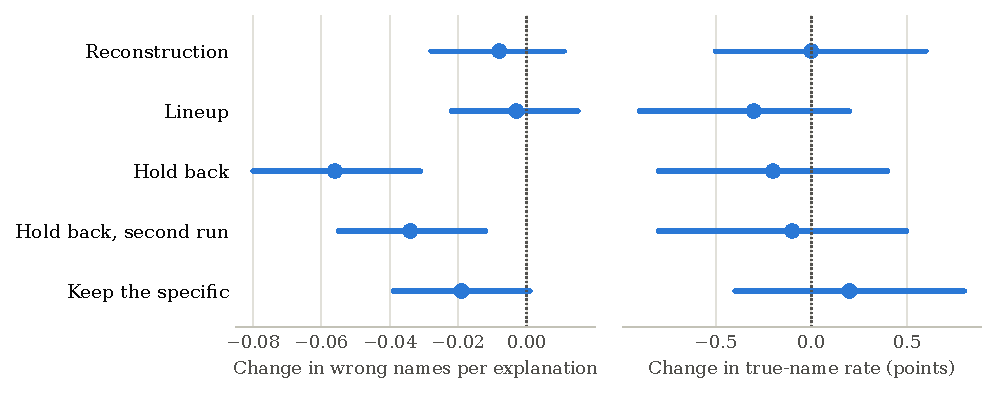
\includegraphics[width=0.92\linewidth]{arms}
\caption[Only the penalty on unsupported names moves wrong names]{Only the penalty on unsupported names
moves wrong names, in both runs, and nothing moves true names. Change relative to the released verbalizer; lines are 95\%
intervals. Natural text, held-out passages.}
\label{fig:arms}
\end{figure}

Both predictions hold (Table~\ref{tab:arms}, Figure~\ref{fig:arms}).

\textbf{More reconstruction changes nothing.} Three further rounds on the original objective leave wrong
names where they were ($-1.3\%$, interval spanning zero). Making reconstruction harder with the lineup does
not help either ($-0.5\%$).

\textbf{A cost on unsupported names removes some of them.} Hold back cuts wrong names by 8.4\%, with an
interval well clear of zero. A second run from a different seed, with its own training passages and
samples, cuts them by 5.1\%, again clear of zero. In both runs the true-name rate, the reconstruction cosine
and the length of the explanations are unchanged, so the verbalizer has not simply learned to name less.

\textbf{The specific cannot be coaxed back.} Rewarding the true name does not raise the true-name rate: $+0.2$
points overall, and $-0.7$ points on the entities held out of training (Table~\ref{tab:keep}). The samples it
was trained on named the true entity 56\% of the time against 45\% on average, yet the trained verbalizer
stays at 45\%.

\begin{table}[t]
\centering
\small
\begin{tabular}{@{}lll@{}}
\toprule
Entities & \shortstack[l]{Change in\\true-name rate\\(points)} & \shortstack[l]{Change in\\wrong names\\per\\explanation} \\
\midrule
Trained on (48) & $+$0.5 {\scriptsize[$-$0.2, $+$1.1]} & $-$0.017 {\scriptsize[$-$0.039, $+$0.006]} \\
Held out of training (12) & $-$0.7 {\scriptsize[$-$2.2, $+$0.9]} & $-$0.028 {\scriptsize[$-$0.072, $+$0.014]} \\
\bottomrule
\end{tabular}

\caption[Keep the specific, by whether the entity was seen in training]{The keep-the-specific verbalizer
against the released one, split by whether the entity was seen in training. Natural text, held-out
passages; 95\% intervals.}
\label{tab:keep}
\end{table}

\section{Analysis}

\textbf{Why the hold-back effect is small.} The samples chosen for training had 35\% fewer wrong names than
average; the trained verbalizer writes 5 to 8\% fewer. Imitating a slightly better subset of one's own samples is
a weak push, because the verbalizer already finds those samples likely. Training harder on the same samples
does not help: five passes over the first round's choices fit them far more closely but gave a smaller
held-out effect ($-6.5\%$), which is memorisation.

\textbf{Why the specific does not come back.} When one of eight samples names the right entity far from it,
that sample looks like a lucky draw, not a skill. A skill would transfer to new passages after training; a
lucky draw does not. This fits Chapter~\ref{ch:fading}: at
16 tokens the information the probe reads is real, but the verbalizer has no reliable way to reach it.
Dingeto~\cite{dingeto2026recap} reports the same for a direct truth reward in a different setting.

\textbf{Filter or fine-tune?} Table~\ref{tab:combine} puts the two fixes side by side. The agreement filter
alone removes 44 to 62\% of the wrong names, depending on distance. Hold back removes 5 to 8\% overall. Together
they are only slightly better than the filter alone.

\begin{table}[t]
\centering
\footnotesize
\setlength{\tabcolsep}{4pt}
\begin{tabular}{@{}cllll@{}}
\toprule
\shortstack[l]{Tokens after\\entity} & Released & Hold back & \shortstack[l]{Released,\\filtered} & \shortstack[l]{Hold back,\\filtered} \\
\midrule
0 & 0.719 {\scriptsize[0.627, 0.813]} & 0.667 {\scriptsize[0.584, 0.755]} & 0.387 {\scriptsize[0.321, 0.454]} & 0.360 {\scriptsize[0.304, 0.416]} \\
1 & 1.097 {\scriptsize[0.954, 1.249]} & 1.006 {\scriptsize[0.876, 1.143]} & 0.609 {\scriptsize[0.508, 0.715]} & 0.554 {\scriptsize[0.463, 0.650]} \\
4 & 0.517 {\scriptsize[0.432, 0.605]} & 0.462 {\scriptsize[0.382, 0.547]} & 0.232 {\scriptsize[0.182, 0.283]} & 0.210 {\scriptsize[0.163, 0.263]} \\
16 & 0.334 {\scriptsize[0.268, 0.409]} & 0.309 {\scriptsize[0.250, 0.373]} & 0.126 {\scriptsize[0.099, 0.156]} & 0.119 {\scriptsize[0.088, 0.150]} \\
\bottomrule
\end{tabular}

\caption[The filter and fine-tuning compared]{Wrong names per explanation with fine-tuning (the first hold-back run),
with the two-of-four agreement filter, and with both. Natural text, held-out passages; 95\% intervals.}
\label{tab:combine}
\end{table}

Larger changes to training, such as a grounding reward~\cite{hong2026grounding} or a different
reconstruction objective~\cite{lek2026flownla}, may well do more. The fine-tuning here matters less as a fix
than as a test. The account in Chapter~\ref{ch:incentives} said what
would happen under each reward, and that is what happened.
